\documentclass
[   twoside=false,     % Einseitiger oder zweiseitiger Druck?
    fontsize=12pt,     % Bezug: 12-Punkt Schriftgröße
    DIV=15,            % Randaufteilung, siehe Dokumentation "KOMA"-Script
    BCOR=17mm,         % Bindekorrektur: Innen 17mm Platz lassen. Copyshop-getestet.
%    headsepline,
    headsepline,  % Unter Kopfzeile Trennlinie (aus: headnosepline)
    footsepline,  % Über Fußzeile Trennlinie (aus: footnosepline)
    open=right,        % Neue Kapitel im zweiseitigen Druck rechts beginnen lassen
    paper=a4,          % Seitenformat A4
    abstract=true,     % Abstract einbinden
    listof=totoc,      % Div. Verzeichnisse ins Inhaltsverzeichnis aufnehmen
    bibliography=totoc,% Literaturverzeichnis ins Inhaltsverzeichnis aufnehmen
    titlepage,         % Titelseite aktivieren
    headinclude=true,  % Seiten-Head in die Satzspiegelberechnung mit einbeziehen
    footinclude=false, % Seiten-Foot nicht in die Satzspiegelberechnung mit einbeziehen
    numbers=noenddot   % Gliederungsnummern ohne abschließenden Punkt darstellen
]   {scrreprt}         % Dokumentenstil: "Report" aus dem KOMA-Skript-Paket
\usepackage{float}
\usepackage{play}
\usepackage[active]{srcltx}
\usepackage[table,xcdraw]{xcolor}
\usepackage{longtable}
\usepackage{subfigure}  	
%\usepackage[activate=normal]{pdfcprot} % Optischer Randausgleich -> pdflatex!
\usepackage{ifthen}
\usepackage[ngerman]{babel}   % Neue Deutsche Rechtschreibung
%\usepackage[latin1]{inputenc} % Zeichencodierung nach ISO-8859-1
\usepackage[utf8]{inputenc}   %	Zeichencodierung nach UTF-8 (Unicode)
\usepackage[T1]{fontenc}
%\usepackage{ae} % obsolet und durch lmodern ersetzt
\usepackage{lmodern}
\usepackage[T1]{url}
\usepackage[final]{graphicx}
\RequirePackage{scrlfile}
\ReplacePackage{scrpage2}{scrlayer-scrpage}
% old: \usepackage[automark]{scrpage2}
\usepackage[automark]{scrlayer-scrpage}
\usepackage{setspace}
\usepackage{cite}
%\usepackage[first,light]{draftcopy} % Für Probedruck
\usepackage[plainpages=false,pdfpagelabels,hypertexnames=false]{hyperref}

% Tiefe der Kapitelnummerierung beeinflussen
\setcounter{secnumdepth}{3} % Tiefe der Nummerierung
\setcounter{tocdepth}{3}    % Tiefe des Inhaltsverzeichnisses

% Hier in die zweite geschweifte Klammer jeweils
% die persönlichen Daten und das Thema der Arbeit eintragen:
\newcommand{\artderausarbeitung}{Hausarbeit}
\newcommand{\namedesautors}{Jonathan Skopp}
\newcommand{\themaderarbeit}{Die Dystopie von Nier - \\ Künstliche Intelligenz und humanoide Roboter in Bezug auf die Entwicklung der Menschheit}

% PDF Metadaten definieren
\hypersetup{
   pdftitle={\themaderarbeit},
   pdfsubject={\artderausarbeitung},
   pdfauthor={\namedesautors},
   pdfkeywords={\artderausarbeitung; TU-Ilmenau; Hausarbeit;}}


% Abkürzungsverzeichnis beeinflussen. Hier nichts ändern!
\usepackage[intoc]{nomencl}
  \AtBeginDocument{\setlength{\nomlabelwidth}{.25\columnwidth}}
  \let\abbrev\nomenclature
  \renewcommand{\nomname}{Abkürzungsverzeichnis}
  \renewcommand{\nomlabel}[1]{#1 \dotfill}
  \setlength{\nomitemsep}{-\parsep}
  \makenomenclature

\usepackage[normalem]{ulem}
  \newcommand{\markup}[1]{\textbf{#1}}

% Seitenlayout festlegen. Hier nichts ändern!
\pagestyle{scrplain}
\ihead[]{\headmark}
\ohead[]{\pagemark}
\chead[]{}
\ifoot[]{}
\ofoot[]{\scriptsize \artderausarbeitung\ \namedesautors}
\cfoot[]{}
\renewcommand{\titlepagestyle}{scrheadings}
\renewcommand{\partpagestyle}{scrheadings}
\renewcommand{\chapterpagestyle}{scrheadings}
\renewcommand{\indexpagestyle}{scrheadings}

% Abschnittsweise Nummerierung anstatt fortlaufend. Hier nichts ändern!
\makeatletter
\@addtoreset{equation}{chapter}
\@addtoreset{figure}{chapter}
\@addtoreset{table}{chapter}
\renewcommand\theequation{\thechapter.\@arabic\c@equation}
\renewcommand\thefigure{\thechapter.\@arabic\c@figure}
\renewcommand\thetable{\thechapter.\@arabic\c@table}
\makeatother

% Quelltextrahmen, klein. Hier nichts ändern!
\newsavebox{\inhaltkl}
\def\rahmenkl{\sbox{\inhaltkl}\bgroup\small\renewcommand{\baselinestretch}{1}\vbox\bgroup\hsize\textwidth}
\def\endrahmenkl{\par\vskip-\lastskip\egroup\egroup\fboxsep3mm%
\framebox[\textwidth][l]{\usebox{\inhaltkl}}}

% Quelltextrahmen, normale Groesse. Hier nichts ändern!
\newsavebox{\inhalt}
\def\rahmen{\sbox{\inhalt}\bgroup\renewcommand{\baselinestretch}{1}\vbox\bgroup\hsize\textwidth}
\def\endrahmen{\par\vskip-\lastskip\egroup\egroup\fboxsep3mm%
\framebox[\textwidth][l]{\usebox{\inhalt}}}

% Trennvorschläge für falsch getrennte Wörter.
% Wird häufig bei eingedeutschen Wörtern benötigt, da LaTeX hierbei
% gerne falsch trennt. Alternativ kann auch im Fliesstext ein
% Trennvorschlag per "\-" hinterlegt werden, bspw.:
% Die Hard\-ware besteht aus A und B.
\hyphenation{
Hard-ware
}

% Sonstige Befehlsdefinitionen hier ablegen.
\newcommand{\entspricht}{\stackrel{\wedge}{=}}

% Tabellenspaltendefinitionen mit fester Breite --> somit Zeilenumbruch innerhalb einer Zelle möglich
% aus http://www.torsten-schuetze.de/tex/tabsatz-2004.pdf
\usepackage{array, booktabs}
\newcolumntype{f}{>{$}l<{$}}
\newcolumntype{n}{>{\raggedright}l}
\newcolumntype{N}{>{\scriptsize}l}
\newcolumntype{v}[1]{>{\raggedright\hspace{0pt}}m{#1}}
\newcolumntype{V}[1]{>{\scriptsize\raggedright\hspace{0pt}}m{#1}}
\newcolumntype{Z}[1]{>{\raggedright\centering}m{#1}}
\newcolumntype{k}[1]{>{\raggedright}p{#1}}
% ergibt Tabllenspalte fester Breite, linksbündig
% Umbruch innerhalb der Zelle mit \\, neue Tabellezeile mit \tabularnewline
% \addlinespace für Gruppentrennung (aus \texttt{booktabs.sty})


\begin{document}
\onehalfspacing
%% ++++++++++++++++++++++++++++++++++++++++++++++++++++++++++++
%% Hauptdatei, Wurzel des Dokuments
%% ++++++++++++++++++++++++++++++++++++++++++++++++++++++++++++
%
%  Gerüst:
%  * Version 0.13
%  * M. Sc. Silvia Krug, silvia.krug@tu-ilmenau.de
%  * Fachgebiet Kommunikationsnetze, TU Ilmenau
%
%  Für Hauptseminare, Studienarbeiten, Diplomarbeiten
%
%  Autor           : Max Mustermann
%  Letzte Änderung : 04.12.2015
%

\begin{titlepage}
\centering

\includegraphics[scale=0.5]{bilder/tui_logo}\\[3ex]
{\Large \textsc{Technische Universität Ilmenau}}\\[3ex]
{\Large Fakultät für Elektrotechnik und Informationstechnik}\\[3ex]
\vfill
{\Large \textbf{\artderausarbeitung}}\\[4ex]
{\large \textbf{\themaderarbeit}}\\[5ex]
\vfill
\begin{tabular}{rl}
\hline\\
vorgelegt von:          & \quad \namedesautors\\[1,5ex]
eingereicht am:         & \quad 31.\,12.\,2011\\[1,5ex]
geboren am:             & \quad 31.\,12.\,1985 in Ilmenau\\[1,5ex]
Studiengang:            & \quad Ingenieurinformatik\\[1,5ex]
Studienrichtung:        & \quad Multimediale Informations- und\\[1,5ex]
                        & \quad Kommunikationssysteme\\[5ex]
Anfertigung im Fachgebiet:
                        & \quad Kommunikationsnetze\\[1,5ex]
                        & \quad Fakultät für Elektrotechnik und Informationstechnik\\[1,5ex]
Verantwortlicher Professor:
                        & \quad Prof.~Dr.~rer.~nat.~Jochen Seitz\\[1,5ex]
Wissenschaftlicher Betreuer:
                        & \quad M.~Sc.~Vorname Nachname
\end{tabular}
\vfill
\end{titlepage}








%% ++++++++++++++++++++++++++++++++++++++++++++++++++++++++++++
%% Hauptdatei, Wurzel des Dokuments
%% ++++++++++++++++++++++++++++++++++++++++++++++++++++++++++++
%
%  Gerüst:
%  * Version 0.13
%  * Skopp Jonathan, jonathan.skopp@gmail.com	
%  * Fakultät IA, TU Ilmenau
%
%  Für Hauptseminare, Studienarbeiten, Diplomarbeiten, Studium Generale
%
%  Autor           : Jonathan, Skopp
%  Letzte Änderung : 09.05.2019
%

\section*{Danksagung}
\ldots 
	
	Folgende Hausarbeit entstand im Rahmen des Studium Generale Wissenschaft und Technik in Utopien im Sommersemester 2019 an der Technischen Universität Ilmenau. Ich bedanke mich bei allen Menschen, die mir durch ihre fachliche und persönliche Hilfe zu einem Gelingen der Arbeit verholfen haben. Ebenso gilt mein Dank auch denen, die mich rund um die Arbeit unterstützt haben. Besonders erwähnenswert ist dabei meine Freundin.
	
	\vspace{10px}
	
	
	
	The following academic paper was written in the summer semester of 2019 at the Technical University of Ilmenau as part of the \dq Studium Generale Wissenschaft und Technik in Utopien \dq . I would like to thank all the people who helped me to make this work a success through their professional and personal help. My thanks also go to all those who helped me with my work. Special thanks to my girlfriend.
	
	
\ldots


%% ++++++++++++++++++++++++++++++++++++++++++++++++++++++++++++
%% Zusammenfassung, Abstract
%% ++++++++++++++++++++++++++++++++++++++++++++++++++++++++++++


\renewcommand{\abstractname}{Kurzfassung}
\begin{abstract}
\ldots \emph{Hier später die eigene deutsche Kurzfassung einfügen}\ldots
\par{}
Dieses Dokument soll als Gerüst für eigene \LaTeX\ Dokumente dienen und
gleichzeitig Beispiele für häufig verwendete Konstrukte wie Tabellen,
Formeln oder Grafiken liefern. Es empfielt sich, diese Elemente per
Cut\&Paste zu kopieren und einzufügen.
\end{abstract}

\renewcommand{\abstractname}{Abstract}
\begin{abstract}
\ldots \emph{Please insert your english abstract here}\ldots
\end{abstract}



% Inhaltsverzeichnis
\cleardoublepage % Seitenumbruch erzwingen vor Änderung des Nummerierungsstils
\pagenumbering{roman} % Nummerierung der Seiten ab hier: i, ii, iii, iv...
\pagestyle{scrheadings} % Ab hier mit Kopf- und Fusszeile
\tableofcontents

% Die einzelnen Kapitel
\cleardoublepage % Seitenumbruch erzwingen vor Änderung des Nummerierungsstils
\pagenumbering{arabic} % Nummerierung der Seiten ab hier: 1, 2, 3, 4...
\chapter{Erklärungen}
\section{Dystopie}
Eine Dystopie bildet in der Wissenschaft das Gegenteil der Utopie. Es ist folglich eine Handlung (meist fiktional) mit einem schlechten Ausgang. Die Gesellschaft in einer solchen Dystopie hat sich nicht wie in einer Eutopie zum Besseren entwickelt, sondern vielmehr zum schlechteren hin. 	



\section{Künstliche Intelligenz}
Künstliche Intelligenz ist das Gebilde und die dadurch resultierende Möglichkeit eines humanoiden Wesens, durch elektronisch Bauteile das Verhalten des menschlichen Gehirns zu imitieren um so eigen abstrakt denken zu können und so eigene logische Resultate herausfinden zu können. Folglich bietet eine Matrix aus digitalen Neuronen die Grundlage der künstlichen Intelligenz. Welche selber kein Objekt oder Tätigkeit ist sondern letztendlich ein Zustand in der sich eine Maschine befinden kann um eigenständig denken zu können.

\section{Turing Test}
 Der Turing Test ist eine Möglichkeit zu entscheiden, ob das vorliegende Subjekt eine menschliche oder eine künstliche Intelligenz ist. Durch geschicktes Fragen kann herausgefunden werden, ob mit der Maschine oder einem Menschen kommuniziert wird. 

\section{Nier:Automata}
Nier:Automata (im Folgenden "Nier" genannt) bildet die Grundlage der hier vorliegenden Hausarbeit. Nier ist ein Action basiertes Videospiel, welches im Jahr 11945 spielt. Folglich hat sich die Welt sehr stark verändert und künstliche Intelligenzen mit Emotionen in Menschenform bilden die Grundlage der Charaktere. 




\input{Künstliche_Intelligenz.tex}
%% ++++++++++++++++++++++++++++++++++++++++++++++++++++++++++++
%% Kapitel 3: Allgemeine Hinweise
%% ++++++++++++++++++++++++++++++++++++++++++++++++++++++++++++
%
%  Gerüst:
%  * Version 0.11
%  * Skopp, Jonathan, jonathan.skopp@gmail.com	
%  * Fakultät IA, Studium Generale
%
%  Für Hauptseminare, Studienarbeiten, Diplomarbeiten, Studium Generale
%
%  Autor           : Jonathan Skopp
%  Letzte Änderung : 31.12.2011
%

\chapter{Der Turing Test}

\section{Alan Turing}
Alan Mathison Turing wurde am 23. Juni 1912 in London geboren. Er wirkte als Kryptologe, Mathematiker und Informatiker. Turing war an vielen technischen Entwicklungen seiner Zeit beteiligt, so unter anderem auch an der nach ihm benannten Turing Maschine. Diese modelliert auf einfachste Weise die Arbeitsmethodik eines Computers. Eingeführt wurde sie bereits 1936. Zu diesem Zeitpunkt war Turing erst 24 Jahre alt. Als Brite war er unter anderem an der Dechiffrierung der deutschen Funksprüche beteiligt. Diese nutzten sie seit 1918. Im Jahr 1950 entwickelte Turing den bekannten Turing-Test. Durch diesen Test soll herausgefunden werden, ob ein Gegenüber ein Mensch oder ein Roboter ist. Wie dieser Test abläuft wird später genauer erklärt. Da Homosexualität unter Georg VI noch unter Strafe stand, wurde Turing 1952 verhaftet und zu einer chemischen Kastration verurteilt. Er starb daraufhin an  Depressionen. ~\cite{Turing_Leben}

\section{Der Turing Test}
Der Grundaufbau des Testes ist eigentlich recht simpel. Obwohl es mehrere Versionen und Arten gibt, bleibt die Grundidee immer gleich. Es gibt eine künstliche Intelligenz (welche es zu testen gilt), einen menschliche Intelligenz und einen menschlichen Prüfer. Der Prüfer hat keinen Kontakt zu den beiden Individuen. Ausschließlich über jeweils eine Tastatur kann er zu den Subjekten Kontakt aufnehmen und sich unterhalten. Heutzutage wird auch, dank der fortschreiten Technik, über eine Audiokommunikation nachgedacht. Der Prüfer unterhält sich nun mit beiden Individuen, um herauszufinden, bei welcher es sich um eine künstliche Intelligenz handelt und bei welcher es sich um einen Menschen handeln könnte. Kann dieser nicht eindeutig herausfinden wer die Maschine ist und wer der Mensch ist, gilt der Test als bestanden. ~\cite{gregorlüdi/martinlüscher20077}

\section{Kritik am Turing Test}
Mit der Zeit werden auch immer mehr Stimmen laut die den Turingtest für überholt und für zu fehlerhaft halten. Laut John Searle zeigt der Test legendlich die Funktionalität der KI auf. Jedoch nicht, dass die Intelligenz wirklich ein Bewusstsein entwickelt und auch nicht dass sie ihre Gedanken auf ein Ziel reflektieren kann. ~\cite{jaai2019}

\section{Alternativen}
Durch den Wandel der Technik bildeten sich auch andere Methoden zur Überprüfung von künstlicher Intelligenz heraus. Diese werden hier nur kurz aufgeführt. 
\begin{description}
	\item[Metzinger-Test]
		Die KI muss hier um den Test zu bestehen nicht nur logisch antworten, sondern auch eigene Thesen formulieren und diese dann auch sinnvoll vertreten. Diese müssen jedoch auch auf Grund der eigenen Fähigkeiten begründet und fundiert sein. 
	\item[Lovelace-Test] In diesem Test muss eine künstliche Maschine originäre Leistungen erbringen. Das heißt, sie muss etwas erschaffen, für das sie nicht programmiert wurde. 
\end{description}


%% ++++++++++++++++++++++++++++++++++++++++++++++++++++++++++++
%% Kapitel 3: Allgemeine Hinweise
%% ++++++++++++++++++++++++++++++++++++++++++++++++++++++++++++
%
%  Gerüst:
%  * Version 0.11
%  * Skopp, Jonathan, jonathan.skopp@gmail.com
%  * Fakultät IA, TU Ilmenau
%
%  Für Hauptseminare, Studienarbeiten, Diplomarbeiten, Studium Generale
%
%  Autor           :   Jonathan Skopp
%  Letzte Änderung :  20.05.2019
%

\chapter{Nier:Automata}
\section{Der Hintergrund}
Nier:Automata ist ein Action basiertes Rollenspiel, welches am 23.02.2017 aus dem bekannten japanischem Studio Square Enix veröffentlicht wurde. Erhältlich ist es für PlayStation4, Windows (PC), und die XBox-One. Folglich deckt es fast den gesamten Markt ab und erfreut sich extrem großer Spielerzahlen. Aufgrund eines hohen Gewaltpotentials sowie recht schwer zu verstehenden Dialogen, ist das Spiel in Deutschland mit FSK 16 an den Start gegangen. Der 2te Teil von Nier (Nier:Automata) spielt im selben Universum wie sein Vorgänger Nier. Das Spiel erreichte sehr gute Kritiken bei diversen Plattformen. Im Vordergrund stehen die menschenähnlichen humanoiden Roboter welche zwar ihren Aufgaben nachgehen und dennoch immer mehr menschliche Emotionen entwickeln.

  \begin{quote}
	Die Figuren, die nicht müde werden, ihre Künstlichkeit zu betonen, dabei aber mehr menschliche Züge zeigen als ihnen lieb sein kann, sorgen dafür, dass ich mit ihnen leide, mit ihnen hasse und mit ihnen hoffe. (Quelle: 4players.de)
	\end{quote}

So schafft Taro Yoko ein weiteres starkes Abenteuer im Nier beziehungsweise Drakengard Stile. Durch tiefe Emotionen wird der Spieler an das Spiel gebunden. Jedoch wird durch actiongeladene Kämpfe, ein sehr gut balanciertes wie auch verstörendes Spiel geschaffen. 
Durch das vorhandensein von insgesamt 26 möglichen Enden ist ein sehr langer Spielspaß garantiert.

\section{Die Hauptcharaktere}

\subsection{Die Androidin 2B}

\begin{quote}
	\dq{Everything that lives is designed to end. We are perpetually trapped...in a never-ending spiral of life and death.}
	(Quelle: 2B in der Prolog Sequenz)
\end{quote}
2B ist die Hauptfigur in der Nier Reihe. Sowohl im ersten wie auch im zweiten Teil ist sie die tragende Figur. Sie ist wie alle anderen YoRHa-Mitglieder eine Androidin, welche mit 9s die Erde von Maschinen befreien muss. Sie soll die Welt von allen "nicht so weit entwickelten" Maschinen befreien und sie so für die Rückkehr der Menschen auf die Erde vorbereiten. Diese leben aktuell auf einer Station auf der Rückseite des Mondes.  2B ist eine sehr pflichtbewusste Androidin. Sie stellt ihre Befehle über alles andere. Sie redet mit anderen Charakteren nicht mehr als wirklich notwendig ist. Ab und zu wirkt sie sehr sardonisch, was sie recht schnell hitzköpfig darstellen lässt. Emotional ist 2B recht kalt. Das ändert sich, je länger sie mit 9S zusammen arbeitet. Anfangs versucht 2B keine Emotionen zuzulassen aber mit 9s Hilfe schafft sie es, diese zuzulassen. Es entwickelt sich über die Zeit eine tiefe Beziehung zu ihm, welche 2B niemals zugeben würde. Dennoch wird diese sehr stark im Kampf gegen \dq Adam und Eva \dq  deutlich denn sie zeigt Eve gegenüber grenzenlosen Hass. Durch den tiefen Konflikt zwischen ihrem Pflichtbewusstsein und den Gefühlen zu 9S wird sie immer mehr hin und hergerissen und entscheidet sich schlussendlich (je nach Ende) für 9S. ~\cite{nier:automatawikia20192b}


\subsection{Der Android 9S}

\begin{quote}
	\dq I‘m not quite sure what it means to mourn, or even if we have a soul to concern ourselves with… But I hope you’re at rest 2B. Sweet dreams. I’ll be with you before long.\dq  \vspace{10px}(9S am Ende B)
\end{quote}
	9S ist im Gegensatz zu 2B nicht für den Kampf vorgesehen. Er ist ein Scanner Android und trägt somit die Aufgabe Informationen und Kartenmaterial zu besorgen. Trotz seiner \dq Einfachheit \dq entwickelt er schneller als 2B Emotionen die Abseits seiner Programmierung liegen. Er ist in fast allen Enden, abgesehen von B, C und D an der Seite von 2B und unterstützt diese. Er ist immer höflich und zuvorkommend. Das spiegelt sich auch in der Anrede von 2B mit \dq Ma'am \dq wieder . Das besondere an 9S ist, das er immer fröhlich und optimistisch ist, wenn er auch gegen Ende seine Emotionen mit 2B zu tauschen scheint. Wie es seiner Programmierung entspricht, ist er ein sehr nützlicher \dq Helfer \dq . 9S Forscherdrang und sein Wunsch, das große Ganze zu sehen, stehen ihm sehr oft im Weg. Leider wird er in fast allen Enden wahnsinnig und 2B ist verpflichtet ihn ziemlich oft zu töten. ~\cite{nier:automatawikia20199S}

\section{Die wichtigsten Nebencharaktere}


\subsection{Adam und Eva}
\begin{quote}
	\dq I—or we machine lifeforms I suppose—have a keen interest in humanity. Love. Family. Religion. War. The more human records I unearth, the more charmed I am by their complexity. This city is one of many areas I've created out of a desire to understand...to know...humans. It's grand, don't you think? Almost...spiritual. And yet, it's nothing more than an android graveyard. I seek to learn and and adopt all facets of humanity! Some desire love! Others family! Only then did I realize the truth...the core of humanity...is conflict. They fight. Steal. Kill. This is humanity in its purest form! \dq (Quelle: Adam zu 2B in der Stadt der Erinnerungen) ~\cite{verschiedene2019npc}
\end{quote}

Adam und sein jüngerer Bruder Eva sind ebenfalls humanoide Androiden. Sie wurden zwischen dem 10. März und dem 7. April 11945 geboren. Folglich sind beide unter einem Jahr alt. Über Eve ist nicht wirklich etwas bekannt. Über Adam hingegen weiss man nur, dass er ziemlich kühl und Herrschsüchtig ist. Abgesehen von den beiden Kampfsequenzen sieht man die beiden meist an einem  Tisch sitzend, ähnlich dem des letzten Abendmahles. Adam ist sehr an den Menschen interessiert und versucht alles, um selber so nah wie möglich selbst einer zu werden. Vor allem seine Expertise über den menschlichen Tot fasziniert ihn. Er versucht ihn oft nach zuempfinden und zu verstehen. Jedoch gelingt ihn das nicht, da er alle \dq Wunden \dq einfach regeneriert. Beide versuchen, wenn auch Eve eher abgelehnt wirkt, trotz ihrer androiden Bauform, Menschen zu werden. Folglich fügt er sich auch selber Schmerzen zu, da Schmerzen auch ein Teil des Menschsein sind. Dennoch wirkt er viel komplexer, tiefer und trauriger als Eve. Er eifert den Menschen nach, ohne die Möglichkeit zu haben, selbst einer zu werden.

\clearpage


\subsection{Die Androidin 2A}
\begin{quote}
	\dq I never quite realized ... how beautiful this world is.\dq \\ (Quelle: 2A am Ende C)
\end{quote}
Auch 2A diente im 14. Maschinenkrieg. Sie ist eine sehr aufbrausende Figur, auch wenn sie sich oft zurückhält und kaum redet. Durch ihre innige Leidenschaft zu kämpfen, gerät sie immer wieder zwischen die Fronten. 2A bringt sich durch unüberlegte und rücksichtlose Handlungen stetig in Gefahr. Als ihr gesamtes Cluster gefallen ist, verliert sie jeglichen Verstand und ihr Verlangen nach Zerstörung allen Lebens nimmt überhand. Trotz allem ist sie nicht ganz ohne Mitgefühl, so hilft sie die Maschinenkinder aus der Fabrik zu retten und tötet 2B auf ihren Wunsch hin. 2A ist einer der widersprüchlichsten Charaktere im gesamtem Spiel. Trotz ihres grenzenlosen Hasses auf alle Maschinen und sonstige Lebensformen, welche sie auch ohne Rückhalt äußert, hilft sie Schwächeren und folgt den Bitten von 2B. 9S hofft bis zum Rindringen in den Marmorturm, das sich 2A von selbst auf ihre eigenen Werte beruft und wieder eine normale humanoide Androidin wird und zu den YoraH Streitkräften zurückkehrt.
 

\section{Die Story}

\subsection{Das Intro}
In dem Intro lernt der Player das Spiel und die Steuerung der Androiden sowie die der Flugzeuge kennen. 2B landet in einer Fabrik wo sie mit Hilfe von 9S eine Maschine der Goliath Klasse zerstören soll. Diese Wesen sind ähnlich wie die Yohrah Androiden mechanisch, jedoch fehlt ihnen jegliche Möglichkeit Empathie zu empfinden. Sie schaden sich und der Umwelt und müssen daher beseitigt werden.

\subsection{Die Mainline}
Das Spiel handelt in einer sehr fernen Zukunft. Die restlichen Menschen wohnen angeblich in einer Kolonisation auf der Rückseite des Mondes. Die Androiden haben nun die Aufgabe die Erde von \dq schlechten, emotionslosen Schrottmonstern \dq zu säubern. Folglich, von allem was nicht menschlich und nicht sie selber sind. Im Laufe des Spieles, treffen die beiden Protagonisten jedoch auf verschiedene Personen beziehungsweise Charaktere, die Zweifel an diesem Leben haben. So wird die kalte und berechenbare 2B immer menschlicher zweifelt an ihren Aufgaben. Bei 9S geht dieser Prozess deutlich schneller. Sie erkennen, dass auch die in den Yorah Augen als feindlichen Goliath Wesen ein eigenes Leben haben. Sie erkennen, das nicht alle böse sind und manche sogar eine eigene Zivilisation aufgebaut haben, in welcher sie die Menschen imitieren. Nun stehen 9S und 2B im Zwiespalt mit dem emotionsbehafteten Maschinen und ihrem Auftraggeber. 

\subsection{Das Ende}
Gegen Ende lernen die Protagonisten die Charaktere Adam und Eva kennen. In der englischen Version heißt sie Eve. Zur Vereinfachung, wird er einfach Eva genannt. Beide eifern den Menschen nach und wollen um jeden Preis welche sein. Auch dann, oder gerade weil sie das Konzept von Tod und Schmerz nicht verstanden haben. 2B und 9S bekämpfen die beiden und gehen schließlich als Sieger hervor. Jedoch sind beide schwer verletzt. Ein einzelnes Ende gibt es nicht. Je nachdem, wie sich der Spieler entscheidet, stehen ihm 26 verschiedene Enden zur Verfügung. 
%% ++++++++++++++++++++++++++++++++++++++++++++++++++++++++++++
%% Kapitel 3: Allgemeine Hinweise
%% ++++++++++++++++++++++++++++++++++++++++++++++++++++++++++++
%
%  Gerüst:
%  * Version 0.11
%  * Skopp, Jonathan, jonathan.skopp@gmail.com	
%  * Fakultät IA, Studium Generale
%
%  Für Hauptseminare, Studienarbeiten, Diplomarbeiten, Studium Generale
%
%  Autor           : Jonathan Skopp
%  Letzte Änderung : 31.12.2011
%
\newpage
\chapter{Dystopie}


\section{Warum sind wir so neugierig nach Utopien?}
Wir sind schon immer daran interessiert wie es in unserer Zukunft aussehen wird. Keiner kann das mit Sicherheit sagen. \\
Verschiedene aktuelle Probleme und Sorgen bringen uns dazu, in der Zukunft danach zu suchen. Schon ganz kindliche Fragen wie \dq Können Autos bald fliegen? \dq könnten der Ursprung einer Dystopie sein. Jeder Gedanke hat die Berechtigung eine Utopie bzw. Dystopie zu werden. Ob nun Eto oder Dysto, dass bleibt dem Erfinder selber überlassen. Fliegende Autos oder Redende Tiere. All das kann eine Zukunfstvision sein. Denn niemand vermag es eindeutig zu beweisen, das es so etwas nicht geben wird. Das es heute noch keine fliegenden Autos gibt, bedarf keines Beweises. Dennoch darf und soll man darüber nachdenken und sich Gedanken machen. ~\cite{dysto}


\section{Warum ist Nier nun eine Dystopie?}
Nier spielt in einer postapokalyptischen Welt, in der es Humanoide gibt. Das eine solche Welt nicht als Wunschvorstellung gilt, sehe ich hier als normal an. Folglich handelt es sich um eine Dystopie. Da das Werk im Jahr 11549 spielt kann man gut erkennen, dass es sich um eine Ferne Zukunft handelt.


\section{Ist so eine Dystopie realistisch ?}
Das wir zur Spielzeit in einer solchen Welt leben ist durchaus denkbar. Durch extreme Misshandlung der Natur kommt es schon heute zu Überflutungen und einer starken Ausbreitung der Wüste. Zum Beispiel ist in den letzten Jahren der Aralsee ausgetrocknet. \\
Jedoch ist zu bezweifeln, dass die Menschheit in naher Zukunft humanoide Roboter entwickeln kann. Auch wenn dies zu wünschen wäre, liegt dieser Wunsch noch in ziemlich weiter Ferne. Der Punkt das wir Roboter brauchen, welche unseren Planeten von gefährlichen Robotern säubern, ist auch gar nicht so weit hergeholt. Produkte wie Siri, Cortana oder ähnliche heute schon das menschliche Verhalten zu imitieren und sich so wie Menschen zu verhalten. Es gibt schon Pflegeroboter wie Paro. Warum sollen wir nicht bald auch Roboter haben, die selber unsere Wohnung aufräumen, putzen oder ähnliches? Doch wie werden sich diese verhalten? Werden sich sich unterwerfen ? Das sind Fragen die erst die Zeit klären kann ? 


\section{Werden Maschinen jemals Gefühle empfinden können?}
Ja. Maschinen werden in der Lage sein, eigene Gefühle zu empfinden. Das wird nicht heute oder morgen passieren, sondern in ferner Zukunft. Dann wäre ein so ähnliches Gespräch wie im Anhang A sehr gut vorstellbar. Dieses Gespräch (hier im original Abgedruckt) stammt aus jenem Werk. Humanoide Androiden werden eigene Gefühle entwickeln, das steht außer Frage. Wie diese sich äußern und welche Form sie annehmen werden, bleibt eine Utopie.


%% ++++++++++++++++++++++++++++++++++++++++++++++++++++++++++++
%% Kapitel 3: Allgemeine Hinweise
%% ++++++++++++++++++++++++++++++++++++++++++++++++++++++++++++
%
%  Gerüst:
%  * Version 0.11
%  * Skopp, Jonathan, jonathan.skopp@gmail.com	
%  * Fakultät IA, Studium Generale
%
%  Für Hauptseminare, Studienarbeiten, Diplomarbeiten, Studium Generale
%
%  Autor           : Jonathan Skopp
%  Letzte Änderung : 31.12.2011
%
\newpage

\chapter{Fazit}
Ich finde es wichtig, dass sich mit dem Thema der humanoiden Roboter beschäftigt wird. Es ist eine unabdingbare Vision der Zukunft. Egal ob man dieser nun ängstlich oder offen gegenübersteht. Roboter bilden die Grundlage des zukünftigen Lebens. Um es mit den Worten von Rene Descarted zu sagen: 
\begin{quote}
	Cogito ergo sum – Ich denke also bin ich.
\end{quote}
Ich denke, also bin ich. Ich selber bin immer ich. Keiner kann mich ersetzen. Sollte die Zeit eintreten, das humanoide Roboter unserer Welt beiwohnen, sollte man diesen nicht mit Angst gegenübertreten. Die Frage, ob sie selber Empathie und Gefühle haben können, beantworte ich hier mit ja. Was unterscheidet uns von Robotern ? Wir sind in allen Aspekten der Maschine unterlegen. Das Einzige was uns über jene Wesen heben soll, ist eine Seele. Diese Nachzubauen ist nicht meine Aufgabe, sondern viel mehr derer, die sich der künstlichen Intelligenz verschrieben haben. Es stellt sich mir jedoch die Frage, ob humanoide Maschinen überhaupt eine solche Seele benötigen? Wenn ja gelten sie als eigenständiges Individuum, welches nicht nur Pflichten sondern auch Rechte bekommen müsste. Hierzu sei auf die Roboterethik verwiesen. Ich freue mich auf ein Zeitalter, in dem wir Hand in Hand mit Robotern leben, die uns und unsere Fähigkeiten um ein vielfaches erweitern. Wir Menschen haben es nie geschafft Frieden auf die Erde zu bringen. Warum also nicht die Aufgabe an klügere Wesen abgeben. Der Mensch sollte dem Humanoid und umgedreht nicht als Feind gegenüberstehen, sondern vielmehr als Freund. Erst wenn alle ihre Angst abgelegt haben, wird ein Zusammenleben möglich sein. Cyborgisierung und Humanoiden sind meiner Meinung nach keine Gefahr für die Menschheit, sondern viel mehr wünschenswert.


\appendix
\part*{Anhang}


% Epilog Pod Dialog


\newpage


\chapter{Epilog der Pod Programme}

\section{Inhalt}
Folgender Dialog erscheint am Ende von \dq Ende E \dq .  Er stellt die Beziehung von 9S zu 2B dar. 	\\
 Der Text ist identisch mit der Version im Spiel. Er wurde hier nur abgedruckt, da er nicht als bekannt vorausgesetzt wird. 


\section{Farmwell}
\subsection{Narration}

\begin{play}
	\speaker{\textbf{Pod 153}} \shortdirection{narration} Everything that lives is designed to end.
	\speaker{\textbf{Pod 153}} \shortdirection{narration} "We" are perpetually trapped ..
	\speaker{\textbf{Pod 153}} \shortdirection{narration} ... in a never-ending spiral of life and death.
	\speaker{\textbf{Pod 153}} \shortdirection{narration} Is this a curse?
	\speaker{\textbf{Pod 153}} \shortdirection{narration} Or some kind of punishment?
	\speaker{\textbf{Pod 153}} \shortdirection{narration}  I often think about the god who blessed us with this cryptic puzzle ...
	\speaker{\textbf{Pod 153}} \shortdirection{narration} ... and wonder if "we'll" ever have the chance to kill him.
\end{play}

\subsection{5. September 11945}

\begin{play}


\speaker{\textbf{Pod 042}}  Unit 2B's vital signs confirmed.

\speaker{\textbf{Pod 042}}  Memory storage, thought circuits, auxiliary motor functions, all confirmed to have been restarted.

\speaker{\textbf{Pod 042}}  Entering reboot sequence.

\speaker{\textbf{2B}}  Ugh ...

\speaker{\textbf{Pod 042}}  Good morning, 2B.

\speaker{\textbf{2B}}  I ...

\speaker{\textbf{Pod 042}}  Report: Unit 2B was killed by unit A2 approximately 1718 hours ago.

\speaker{\textbf{2B}}  1718 hours ago ... So ... 72 days, then.

\speaker{\textbf{Pod 042}}  Following that, us tactical support units reconstructed your parts.

\speaker{\textbf{Pod 042}}  The virus previously inside you deactivated along with the tower's collapse, and remains in suspension. 

\speaker{\textbf{2B}}  Tower ...? What happened ...?

(2B suddenly realizes something.)

\speaker{\textbf{2B}}  Ah!! 9S ...!!

\speaker{\textbf{Pod 153}}  Report: Unit 9S ceased activity approximately 740 hours ago.

\speaker{\textbf{2B}}  Pod ... 153?

\speaker{\textbf{Pod 153}}  Unit 9S was severely contaminated, however said virus deactivated along with the tower's collapse, and remains in suspension.

\speaker{\textbf{2B}}  So he's just ... asleep?

\speaker{\textbf{Pod 153}}  Negative: An error occurred during unit 9S's reboot sequence.

\speaker{\textbf{2B}}  What do you mean, an error ...?

\speaker{\textbf{Pod 153}} \shortdirection{narration} Unknown: All checks were completed, however his personal data will not begin loading procedures, causing an inability to reboot.

\speaker{\textbf{2B}}  His personal data won't load ... Then in that case, run the monitoring sequence, and skip the check sequence ...

\speaker{\textbf{Pod 153}} \shortdirection{narration} Negative: This unit has already attempted 345 combinations 34,500 times, and all have ended in failure.

\speaker{\textbf{Pod 153}} \shortdirection{narration} Unit 9S's current state suggests there is a possibility his personal data has been lost due to some unknown cause.

\speaker{\textbf{2B}}  His personal data is ... lost ...?

\speaker{\textbf{Pod 153}} \shortdirection{narration} Proposal: Unit 2B should consider disposing of unit 9S's body.

(2B speaks in a strong tone.)

\speaker{\textbf{2B}}  There's no way I could ... just dispose of his body ...!

(There is a considerable pause.)

\speaker{\textbf{Pod 153}} \shortdirection{narration} ... Understood.

\speaker{\textbf{2B}} \shortdirection{narration} After being reconstructed, there wasn't even a hint of dirt on 9S's body ...

\speaker{\textbf{2B}} \shortdirection{narration} His face ... looked just like he was sleeping.

\speaker{\textbf{2B}} \shortdirection{narration} I took my weapon in hand, and packed the minimum necessary provisions, before standing up.

\speaker{\textbf{2B}} \shortdirection{narration} I had to go.

\speaker{\textbf{2B}} \shortdirection{narration} There had to be a way to get 9S to reboot properly.

\speaker{\textbf{2B}} \shortdirection{narration} That's what I believed.
\end{play}


\subsection{14. September 11945}
\begin{play}
\speaker{\textbf{2B}} \shortdirection{narration} I received information on what happened while I was gone from the pods.

\speaker{\textbf{2B}} \shortdirection{narration} About A2 ... and 9S.

\speaker{\textbf{2B}} \shortdirection{narration} I also heard about how the two of them destroyed some huge "Tower" that had been created by the machine lifeforms.

\speaker{\textbf{2B}} \shortdirection{narration} The rubble from it is still scattered all throughout the city.

\speaker{\textbf{2B}} \shortdirection{narration} The City Ruins' landscape had been completely changed.

\speaker{\textbf{Pod 042}} \shortdirection{Proposal} Unit 2B should gather information at the resistance camp.

\speaker{\textbf{2B}} \shortdirection{narration} The resistance camp was able to miraculously avoid damage from the collapse of the tower ...

\speaker{\textbf{2B}} \shortdirection{narration} However Devola and Popola, and a few others in the resistance, lost their lives in the fight with the machines.

\speaker{\textbf{2B}} \shortdirection{narration} Even though Anemone was faced with such a difficult situation, she still remained level-headed.

\speaker{\textbf{2B}} \shortdirection{narration} I tried speaking to Anemone about the situation with 9S's rebooting, but she wasn't able to provide me with any helpful information.

\speaker{\textbf{Pod 042}} \shortdirection{Report} Relevant records within the Bunker have been lost.

\speaker{\textbf{2B}} \shortdirection{narration} We YoRHa units are a special type.

\speaker{\textbf{2B}} \shortdirection{narration} We contain something other androids don't within us — a Black Box.

\speaker{\textbf{2B}} \shortdirection{narration} And due to that, we're capable of much higher functionality. 

\speaker{\textbf{2B}} \shortdirection{narration} However, unlike general androids, our maintenance is only able to be done on the Bunker.

\speaker{\textbf{2B}} \shortdirection{narration} It's possible to make easy repairs with the small amount of materials and programs at access points, but detailed information about the insides of our bodies was lost along with the fall of the Bunker.

\speaker{\textbf{2B}} \shortdirection{narration} Even so, I was traveling from place to place looking for the information I needed.

\speaker{\textbf{2B}} \shortdirection{narration} No matter ... how long it took.

\speaker{\textbf{Pod 042}} \shortdirection{Alert} Unit 2B is taking damage due to maintenance failure.

\speaker{\textbf{Pod 042}} \shortdirection{Proposal} Unit 2B should perform proper repair and replenish materials.

\speaker{\textbf{2B}} \shortdirection{narration} With how tired I was, even doing simple first aid felt troublesome.

\speaker{\textbf{2B}} \shortdirection{narration} In the depths of my heart, I started to feel like ... everything I was doing was meaningless.

\speaker{\textbf{2B}} \shortdirection{narration} I don't ... care anymore.

\speaker{\textbf{2B}} \shortdirection{narration} I wonder if ... 9S will ever wake up.

\speaker{\textbf{2B}} \shortdirection{narration} That sort of dark thought process began to take over.

\speaker{\textbf{2B}} \shortdirection{narration} And I shook my head.

\speaker{\textbf{2B}} \shortdirection{narration} I couldn't give up. I couldn't give up. I couldn't give up.

\speaker{\textbf{2B}} \shortdirection{narration} Even if I was just deceiving myself, I couldn't admit that.

\speaker{\textbf{2B}} \shortdirection{narration} It caused my body to become heavy.

\speaker{\textbf{2B}} \shortdirection{narration} If I go further away from here, I may be able to find surviving YoRHa members.

\speaker{\textbf{Pod 042}} \shortdirection{Report} Mail notification received.

\speaker{\textbf{2B}}  ... Check it.

(The pod reads out the mail's contents in its usual tone of voice.)

\speaker{\textbf{Pod 153}}  Sender: Jackass.

\speaker{\textbf{Pod 153}}  Subject: About 9S's Personal Data Reboot.

\speaker{\textbf{Pod 153}}  Yo, how's it going, 2B?

\speaker{\textbf{Pod 153}}  I know a little something about 9S's condition.

\speaker{\textbf{Pod 153}}  I've been looking into a lot of things since everything happened, and I came across some concerning information.

\speaker{\textbf{Pod 153}}  There were some logs remaining in the access port outside of 9S's memory storage.

\speaker{\textbf{Pod 153}}  They were a communication record from the "Ark" object those machine lifeforms made.

\speaker{\textbf{Pod 153}}  I don't know anything about that "Ark" thing, but it might be some sort of server.

\speaker{\textbf{Pod 153}}  I'll send you the time and coordinates that were written in that log right away.

\speaker{\textbf{Pod 153}}  There might be a hint somewhere in them.

(There's a short pause.)

\speaker{\textbf{Pod 153}}  This concludes the body of the email. Time and three-dimensional coordinate data is attached.

\speaker{\textbf{2B}} \shortdirection{narration} Those coordinates ... were right in the area where the Tower collapsed.
	
	
	
\end{play}
\subsection{17. September 11945}
\begin{play}
\speaker{\textbf{2B}} \shortdirection{narration} Mountains and mountains of white rubble, as far as I could see.

\speaker{\textbf{2B}} \shortdirection{narration} I'd arrived at the center of where the Tower collapsed.

\speaker{\textbf{2B}} \shortdirection{narration} And it was there, where I began digging.

\speaker{\textbf{Pod 153}} \shortdirection{Hypothesis} Origin point is 40 meters below the current point.

\speaker{\textbf{Pod 042}} \shortdirection{Proposal} Proposal: Search for a more efficient method for digging.

\speaker{\textbf{2B}} \shortdirection{narration} That's right, the coordinates Jackass sent me pointed right to a location within the Tower's rubble.

\speaker{\textbf{2B}} \shortdirection{narration} I was digging through it so I could reach the position she gave me.

\speaker{\textbf{2B}} \shortdirection{narration} But the material was much more firm than I expected it to be, and my digging wasn't going particularly well.

\speaker{\textbf{2B}} \shortdirection{narration} My breath began to show, and before I'd realized it, it was snowing.

\speaker{\textbf{2B}} \shortdirection{narration} It seems the Tower's rubble was absorbing the surrounding area's heat and causing the area to cool.

\speaker{\textbf{2B}} \shortdirection{narration} According to the pods, it was made of materials derived from the bodies of machine lifeforms, which centered around silicon, among other things.

\speaker{\textbf{2B}} \shortdirection{narration} But that didn't matter.

\speaker{\textbf{2B}} \shortdirection{narration} I only cared about my digging.

\speaker{\textbf{Pod 153}} \shortdirection{Hypothesis} Origin point is 25 meters below the current point.

\speaker{\textbf{Pod 042}} \shortdirection{Proposal} Alert: Unit 2B is taking damage due to maintenance failure.

\speaker{\textbf{2B}} \shortdirection{narration} The Tower's materials became increasingly firm the further down I went.

\speaker{\textbf{2B}} \shortdirection{narration} I was using my weapon to dig, but I had to stop using my one-handed sword to switch to something better suited, and I proceeded downward by practically crushing the materials.

\speaker{\textbf{2B}} \shortdirection{narration} I continued on, my mind devoid of any other thoughts, until I finished.

\speaker{\textbf{2B}} \shortdirection{narration} I could feel an ache run through my pain sensors.

\speaker{\textbf{2B}} \shortdirection{narration} But it was only thanks to that pain that I was able to keep my sanity.

\speaker{\textbf{Pod 153}} \shortdirection{Hypothesis} Origin point is 12 meters below the current point.

\speaker{\textbf{Pod 042}} \shortdirection{Proposal} Alert: Unit 2B is taking damage due to maintenance failure.

\speaker{\textbf{Pod 042}} \shortdirection{Proposal} Alert: If no proper repair is performed, it will cause severe impact to the unit's body.

\speaker{\textbf{2B}} \shortdirection{narration} As I continued to dig, I found out what that "Ark" really was.

\speaker{\textbf{2B}} \shortdirection{narration} It seemed to be a huge memory unit, made by combining complex crystals.

\speaker{\textbf{2B}} \shortdirection{narration} However, as it'd been shattered to pieces, I couldn't find a single "living" crystal.

\speaker{\textbf{2B}} \shortdirection{narration} Regardless, I continued digging in search of the Ark's crystals.

\speaker{\textbf{2B}} \shortdirection{narration} With each swing of my weapon, blood began to scatter.

\speaker{\textbf{2B}} \shortdirection{narration} I couldn't feel my fingertips anymore, and the sensors running from my wrists had died.

\speaker{\textbf{2B}} \shortdirection{narration} The bolts I'd used to forcibly fix it were starting to dig into my skin.

\speaker{\textbf{2B}} \shortdirection{narration} But that didn't matter.

\speaker{\textbf{2B}} \shortdirection{narration} Somewhere up ahead, the information I needed to save 9S was ...

\speaker{\textbf{2B}} \shortdirection{narration} Even if only a little remains of the Ark, I ... I have to ...!!

(An error sound pings.)

\speaker{\textbf{Pod 042}} \shortdirection{Proposal} Alert: Unit 2B entered forced shutdown due to overload.
\end{play}
\subsection{19. September 11945}
\begin{play}
	\speaker{\textbf{Pod 042}}  Emergency nanomachine removal complete.
	
	\speaker{\textbf{Pod 042}}  Unit 2B's vital signs confirmed.
	
	\speaker{\textbf{Pod 042}}  Entering reboot sequence.
	
	(A long "beeeeep" alert sounds.)
	
	(Afterwards, a short three "beeps" sound.)
	
	\speaker{\textbf{Pod 042}}  Good morning, 2B.
	
	\speaker{\textbf{2B}}  Huh? I ...
	
	\speaker{\textbf{Pod 042}}  You entered a forced shutdown due to severe continuous operation.
	
	\speaker{\textbf{2B}} \shortdirection{narration} When I hurriedly asked about the Ark, the pods showed me a small, orange sparkling crystal.
	
	\speaker{\textbf{2B}} \shortdirection{narration} What they found seemed to be a remnant of the machine lifeforms' communication protocol.
	
	\speaker{\textbf{2B}} \shortdirection{narration} If we use that protocol and its data, we could create a key, and open up 9S's memory storage.
	
	\speaker{\textbf{2B}} \shortdirection{narration} Although I didn't understand the details, there was meaning in my continued digging.
	
	\speaker{\textbf{2B}} \shortdirection{narration} The pods siphoned out the data and recombined it to create a repair vaccine.
	
	\speaker{\textbf{2B}} \shortdirection{narration} Then, we could pull the cable from 9S's access port and create a wired connection.
	
	\speaker{\textbf{2B}} \shortdirection{narration} With that, I'd be able to insert the repair vaccine.
	
	\speaker{\textbf{2B}} \shortdirection{narration} After that, all I'd have to do is hope that 9S's memory storage data could be evacuated into his personal data.
	
	\speaker{\textbf{Pod 153}}  Repair vaccine injected.
	
	(Three seconds later, the sound of a heartbeat stops and a flatline beeps.)
	
	\speaker{\textbf{Pod 153}}  No effect. Re-administering repair vaccine.
	
	(Three seconds later, the sound of a heartbeat stops and a flatline beeps.)
	
	\speaker{\textbf{Pod 153}}  No effect. Re-administering repair vaccine.
	
	(Three seconds later, the sound of a heartbeat stops and a flatline beeps.)
	
	\speaker{\textbf{Pod 153}}  No effect.
	
	\speaker{\textbf{2B}}  Why ... Why isn't it ...?!
	
	\speaker{\textbf{Pod 042}} \shortdirection{Hypothesis} Repair vaccine is a failure.
	
	\speaker{\textbf{Pod 153}} \shortdirection{Negative} Repair vaccine's functions confirmed to be normal.
	
	\speaker{\textbf{2B}}  Try it again ... Administer it to him again!
	
	(Three seconds later, the sound of a heartbeat stops and a flatline beeps.)
	
	\speaker{\textbf{Pod 153}}  No effect.
	
	\speaker{\textbf{2B}}  Try ... again ...
	
	\speaker{\textbf{Pod 153}} \shortdirection{Report} Traces detected indicating the memory region of unit 9S's contents have been erased.
	
	\speaker{\textbf{Pod 042}} \shortdirection{Negative} It is an effect of the repair vaccine.
	
	\speaker{\textbf{Pod 042}} \shortdirection{Hypothesis} Unit 9S's personal data has been lost.
	
	\speaker{\textbf{2B}}  His personal data ... is lost ...?
	
	\speaker{\textbf{Pod 042}}  His personal data was wiped of his own accord, but there is the possibility it was moved to a different location.
	
	\speaker{\textbf{Pod 042}}  According to unit A2's records, it is possible his data evacuated using the machine lifeforms' Ark.
	
	\speaker{\textbf{Pod 042}} \shortdirection{Report} Possibility of recovering 9S's personal data extremely low.
	
	S.P.
	
	\speaker{\textbf{2B}}  No ...
	
	(Three beeps suddenly sound.)
	
	\speaker{\textbf{Pod 153}} \shortdirection{Report} Memory components discovered within traces of personal data.
	
	\speaker{\textbf{Pod 153}}  Partial playback possible of memory containing the reason behind his personal data's reparation failure.
	
	\speaker{\textbf{Pod 153}} \shortdirection{Query} Does unit 2B feel it necessary to repair this memory component?
	
	\speaker{\textbf{2B}}  ... Repair it.
	
	\speaker{\textbf{Pod 153}}  Understood.
	
	\speaker{\textbf{Pod 153}}  Data repair complete.
	
	\speaker{\textbf{Pod 153}}  Starting playback.
	
	(9S's voice begins to play back with the sound quality of a radio.)
	
	(He seems to be suffering.)
	
	\speaker{\textbf{9S}}  I didn't ... get on the Ark created by the machine lifeforms.
	
	\speaker{\textbf{9S}}  We YoRHa ... We don't deserve to be loved by this world ... We're just soldiers created to die ...
	
	\speaker{\textbf{9S}}  But I ... I think I'm glad ... that I was born as myself ...
	
	\speaker{\textbf{9S}}  My personal data, it ... it can't keep it's shape any longer.
	
	\speaker{\textbf{9S}}  I wonder if I'm about to disappear ...
	
	\speaker{\textbf{9S}}  But ... I'm okay with that ...
	
	(2B begins crying, without making a sound.)
	
	\speaker{\textbf{9S}}  Hey, 2B ... We're ... we're not immortal or anything.
	
	\speaker{\textbf{9S}}  Someday, we'll break down and return to the Earth.
	
	\speaker{\textbf{9S}}  But, my existence ... It wasn't meaningless ...
	
	\speaker{\textbf{9S}}  Meeting you ... gave meaning to my birth ...
	
	\speaker{\textbf{9S}}  Thank you ...
	
	\speaker{\textbf{9S}}  Thank you ...
	
	(9S's voice becomes hidden behind static.)
	
	(2B begins weeping.)
	
	\speaker{\textbf{2B}}  Nines ...
	
	\speaker{\textbf{Pod 042}} \shortdirection{narration} 2B didn't move from where she was.
	
	\speaker{\textbf{Pod 042}} \shortdirection{narration} She remained there, unmoving ... forever.
	
	\speaker{\textbf{Pod 042}} \shortdirection{narration} It was a completely irrational act.
	
	\speaker{\textbf{Pod 042}} \shortdirection{narration} However, "we" can now understand the reason behind it.
	
	\speaker{\textbf{Pod 042}} \shortdirection{narration} Why it was that 2B didn't move.
	
	\speaker{\textbf{Pod 042}} \shortdirection{narration} Why it was that she didn't speak.
	
	\speaker{\textbf{Pod 042}} \shortdirection{narration} Because "we" are now in that same place, feeling the same thing.
	
	(There is a small pause.)
	
	\speaker{\textbf{Pod 153}} \shortdirection{narration} Everything that lives is designed to end.
	
	\speaker{\textbf{Pod 153}} \shortdirection{narration} "They" are perpetually trapped ...
	
	\speaker{\textbf{Pod 153}} \shortdirection{narration} ... in a never-ending spiral of life and death.
	
	\speaker{\textbf{Pod 153}} \shortdirection{narration} However ... life is all about the struggle within this cycle.
	
	\speaker{\textbf{Pod 153}} \shortdirection{narration} That is what "we" believe. 	
\end{play}

% Literaturverzeichnis einbinden
%% ++++++++++++++++++++++++++++++++++++++++++++++++++++++++++++
%% Anhang: Literaturverzeichnis
%% ++++++++++++++++++++++++++++++++++++++++++++++++++++++++++++


% Mit dem Befehl \nocite werden auch nicht im Text zitierte
% aus der Literaturdatenbank mit in das Literaturverzeichnis aufgenommen.
% Ein "\nocite{*}" übernimmt ungeprüft die komplette Datenbank.
%\nocite{*}

\cleardoublepage
\ihead[]{Literaturverzeichnis}
\bibliographystyle{alphadin}
\bibliography{literatur} % "literatur.bib" ist hier die einzige Literaturdatenbank.

% Alternativ: Mehrere Datenbanken verwenden, falls eine
% oder mehrere umfangreiche Sammlungen exisitieren:
%\bibliography{literatur_buecher,literatur_weblinks}


% Bildersammlung von Nier

\centering
\chapter{Bilder aus Nier:Automata}

\section{Die Welt}

\restylefloat{figure}

\begin{figure}[h!]
	\centering
	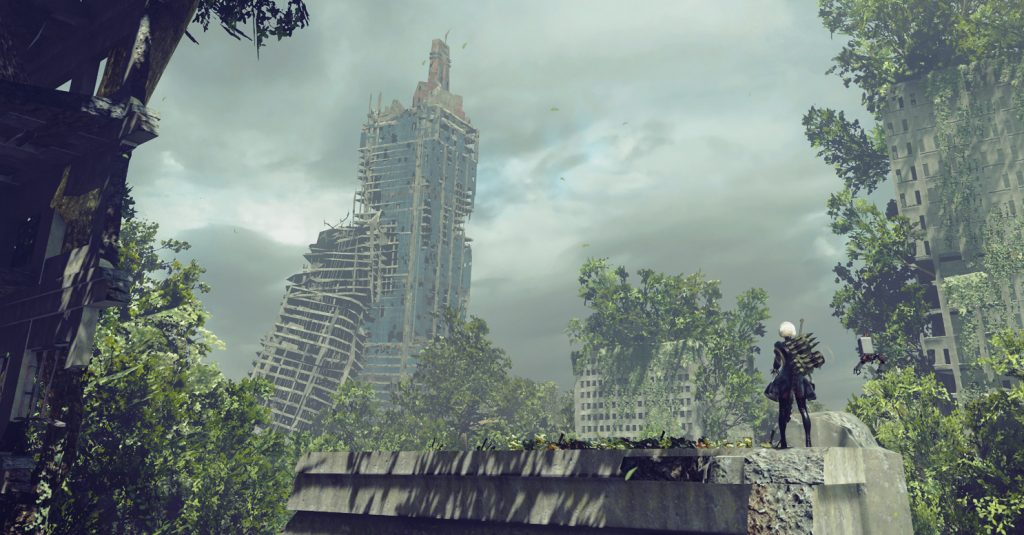
\includegraphics[width=15cm,height=7cm]{Nier/World/area.jpg}
	\caption{Die Ruinenstadt}
	\label{img:passante}
\end{figure}

\begin{figure}[h!]
	\centering
	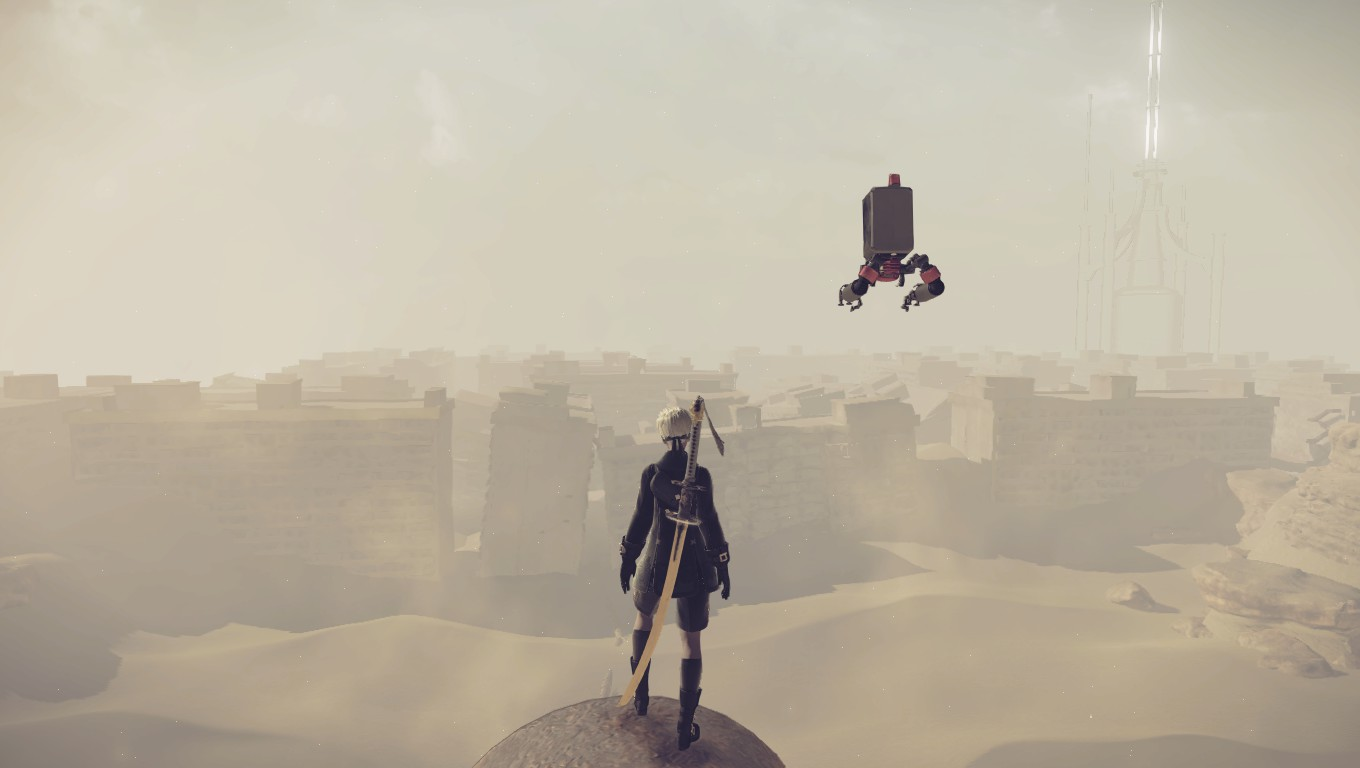
\includegraphics[width=15cm,height=7cm]{Nier/World/desert.jpg}
	\caption{Die Wüste}
	\label{img:passante}
\end{figure}

\begin{figure}[h!]
	\centering
	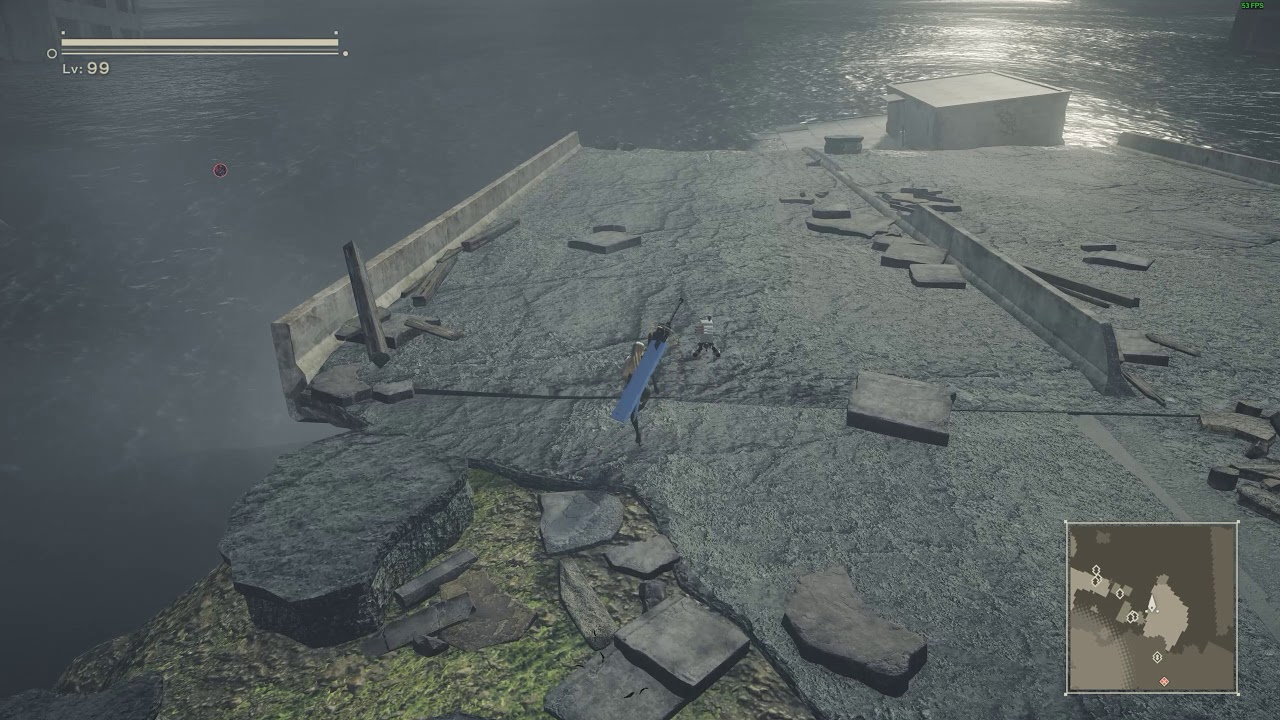
\includegraphics[width=15cm,height=7cm]{Nier/World/water.jpg}
	\caption{Die überflutete Stadt}
	\label{img:passante}
\end{figure}

\begin{figure}[h!]
	\centering
	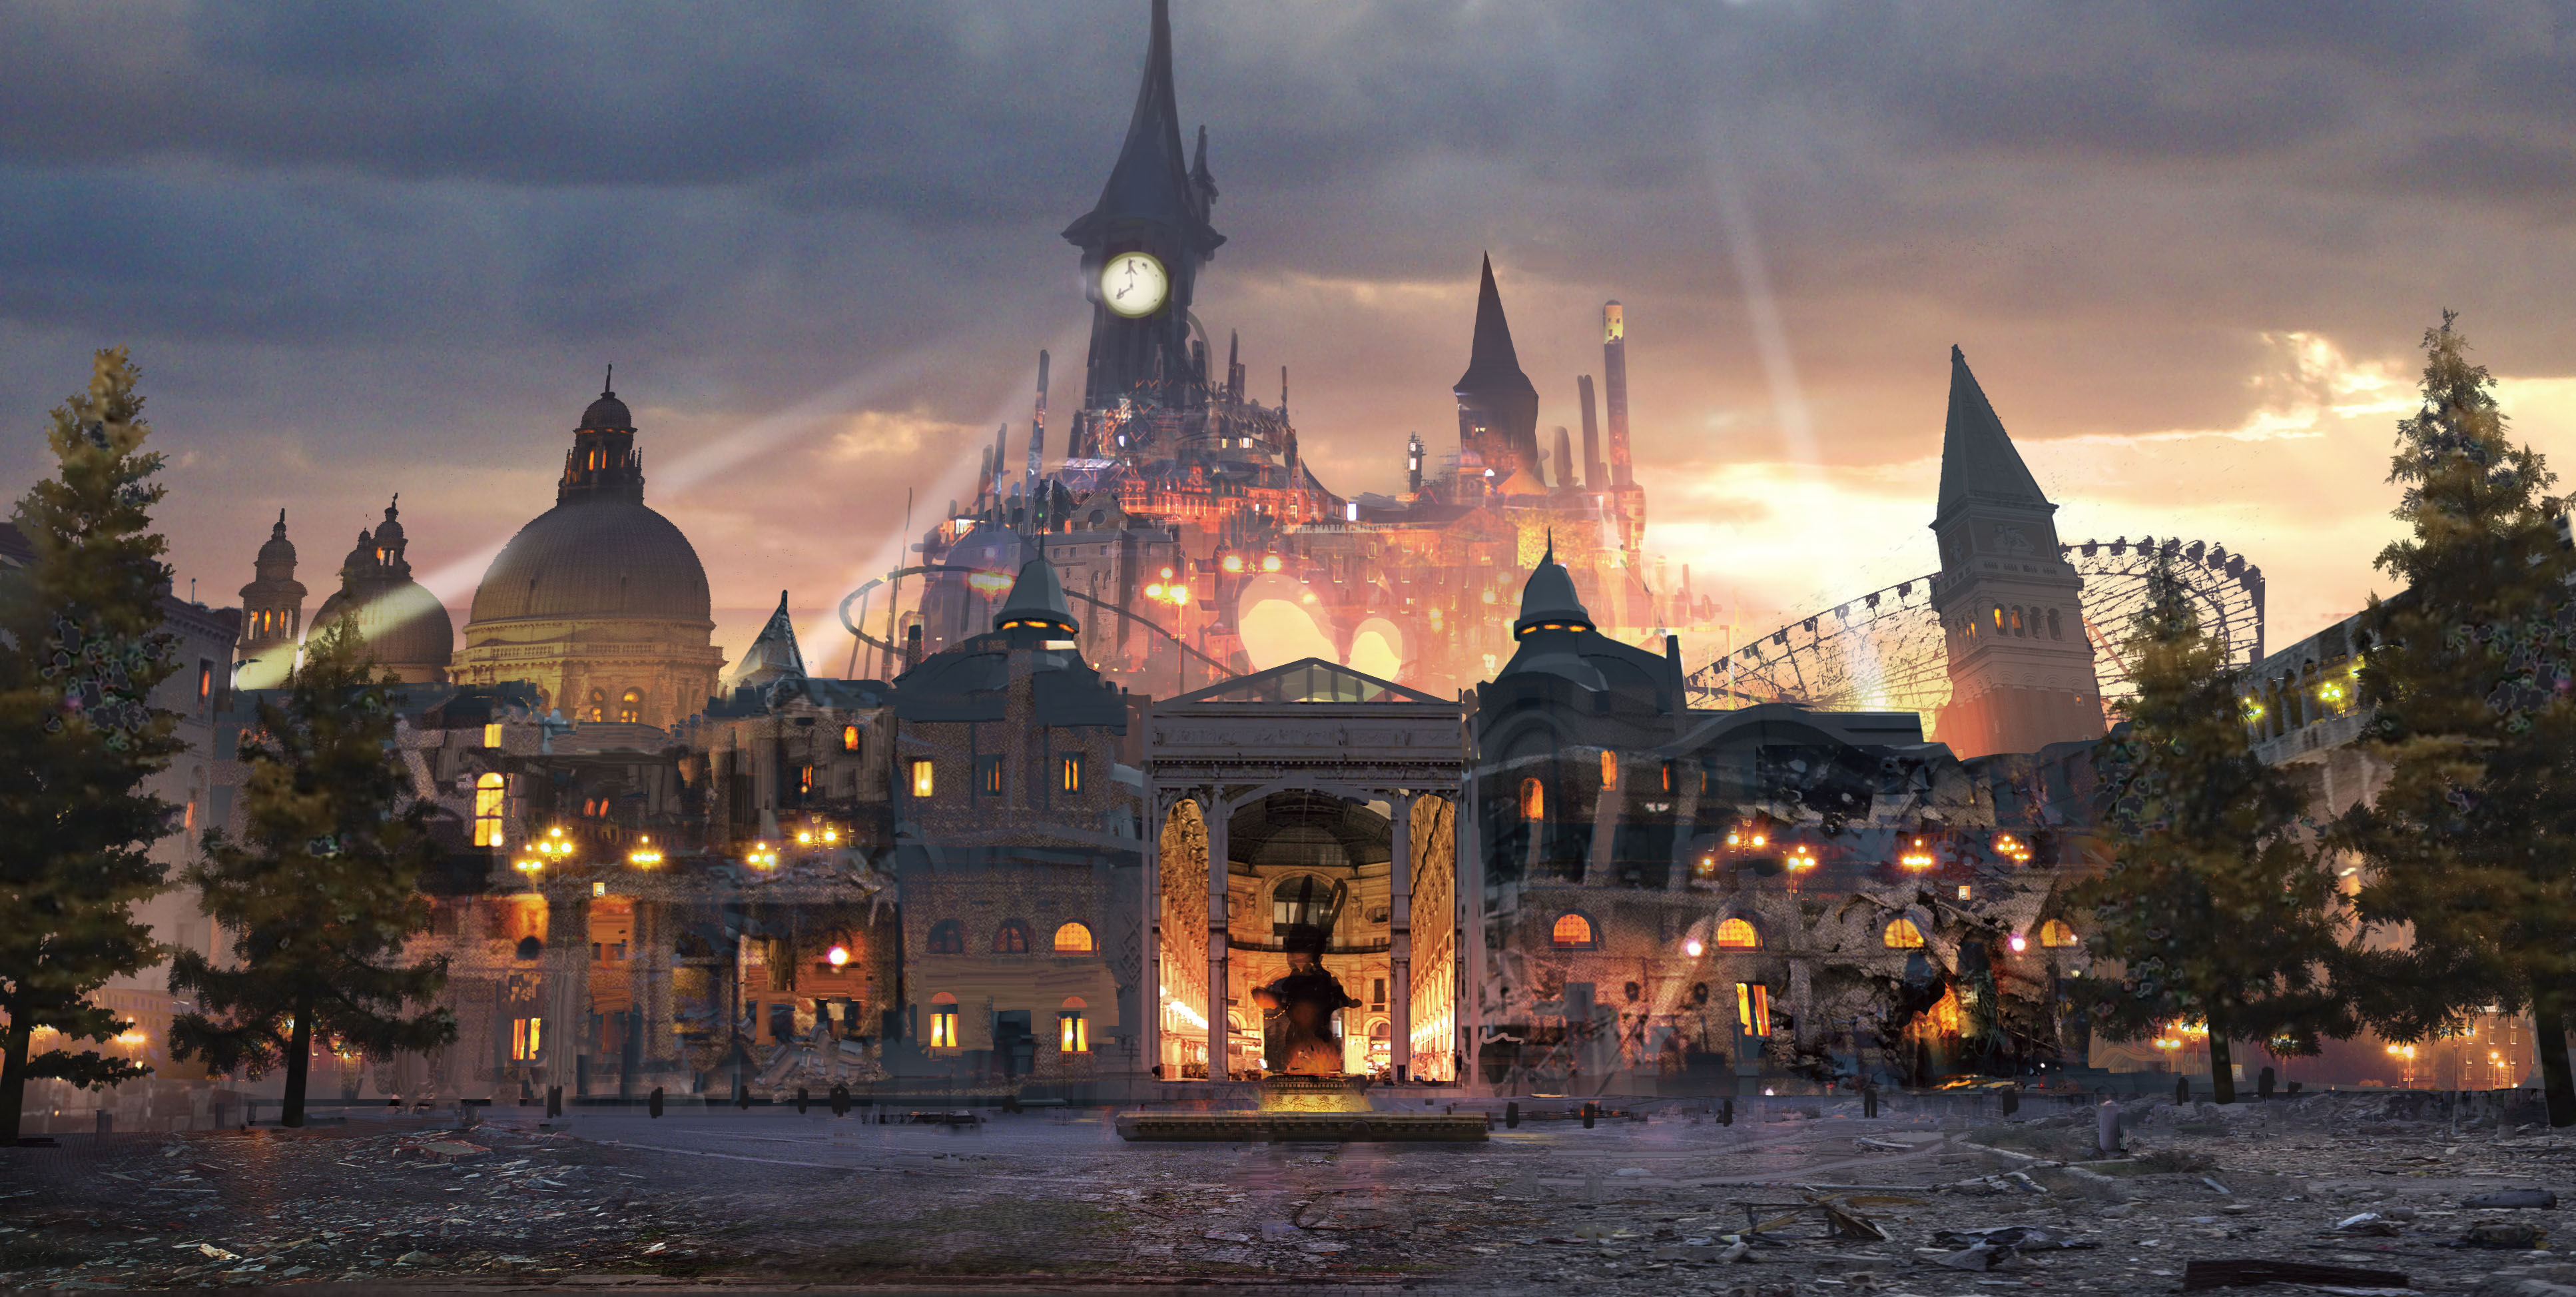
\includegraphics[width=15cm,height=7cm]{Nier/World/fun.jpg}
	\caption{Der Freizeitpark}
	\label{img:passante}
\end{figure}

\clearpage
\section{Die Charaktere}

\begin{figure}[hb!]
	\subfigure[Der humanoide Android 9s]{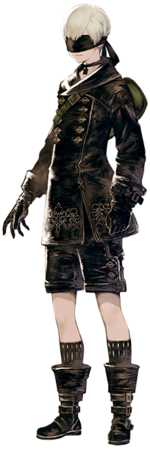
\includegraphics[width=0.49\textwidth,height=17cm]{Nier/Chara/YoRHa_No-9_Type_S.png}} 
	\subfigure[Die humaoide Androidin 2b]{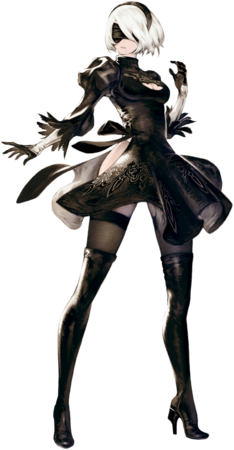
\includegraphics[width=0.49\textwidth,height=17cm]{Nier/Chara/YoRHa_No-2_Type_B.png}} 
	\caption{Die Hauptcharaktere} 
\end{figure}


\clearpage
\section{Wichtige Nebencharaktere}

\begin{figure}[hb!]
	\subfigure[Adam]{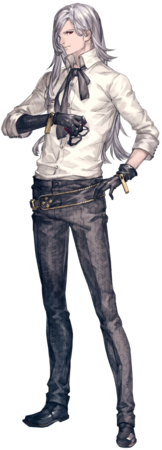
\includegraphics[width=0.49\textwidth,height=17cm]{Nier/Chara/YoRHa_Commander.png}} 
	\subfigure[Die humanoide Androidin 2a]{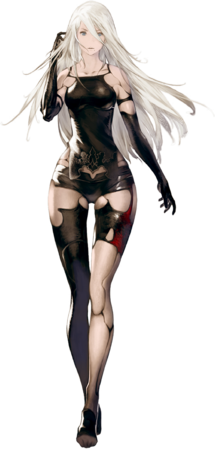
\includegraphics[width=0.49\textwidth,height=17cm]{Nier/Chara/YoRHa_No-2A.png}}
	\caption{Wichtige Nebencharaktere} 
\end{figure}







% Abbildungsverzeichnis einbinden

\cleardoublepage
\ihead[]{Abbildungsverzeichnis}
\listoffigures


% Tabellenverzeichnis einbinden
%%% ++++++++++++++++++++++++++++++++++++++++++++++++++++++++++++
%% Anhang: Tabellenverzeichnis
%% ++++++++++++++++++++++++++++++++++++++++++++++++++++++++++++

% Hier keine weiteren Änderungen vornehmen
\cleardoublepage
\ihead[]{Tabellenverzeichnis}
\listoftables



% Abkürzungsverzeichnis einbinden
%%% ++++++++++++++++++++++++++++++++++++++++++++++++++++++++++++
%% Anhang: Abkürzungsverzeichnis
%% ++++++++++++++++++++++++++++++++++++++++++++++++++++++++++++


% Hier keine weiteren Änderungen vornehmen
\cleardoublepage
\ihead[]{Abkürzungsverzeichnis und Formelzeichen}
\printnomenclature



% Thesen
%% ++++++++++++++++++++++++++++++++++++++++++++++++++++++++++++
%% Thesen zur Ausarbeitung. Für Diplomarbeiten
%% ++++++++++++++++++++++++++++++++++++++++++++++++++++++++++++
%
%  Gerüst:
%  * Version 0.11
%  * Dipl.-Ing. Karsten Renhak, karsten.renhak@tu-ilmenau.de
%  * Fachgebiet Kommunikationsnetze, TU Ilmenau
%
%  Für Hauptseminare, Studienarbeiten, Diplomarbeiten
%
%  Autor           : Max Mustermann
%  Letzte Änderung : 31.12.2011
%

\chapter*{Thesen zur \artderausarbeitung}
\addcontentsline{toc}{chapter}{Thesen zur \artderausarbeitung}
\ihead[]{Thesen zur \artderausarbeitung}

\begin{enumerate}
\item Mit \LaTeX\ gesetzte Dokumente sehen überall
      gleich aus. Sie werden ähnlich wie HTML in Klartext
      geschrieben und anschließend mit Hilfe eines Konverters in
      Postscript- oder PDF"=Dateien gewandelt.
\item \LaTeX\ gibt es für alle wichtigen Betriebssysteme.
\item Die Benutzung einer integrierten Entwicklungsumgebung,
      beispielsweise {\ttfamily Kile} oder {\ttfamily TeXnicCenter},
      wird empfohlen.
\item Dieses Dokument ist Formatvorlage und Einstiegshilfe
      zugleich. Einfach den Text durch die eigene Ausarbeitung
      ersetzen.
\end{enumerate}

% Etwas Platz schaffen:
\section*{}

Ilmenau, den 31.\,12.\,2011\hfill \namedesautors


% Abschlusserklärung

\chapter*{Erklärung}
\addcontentsline{toc}{chapter}{Erklärung}
\ihead[]{Erklärung}

Die vorliegende Arbeit habe ich selbstständig ohne Benutzung anderer als der
angegebenen Quellen angefertigt. Alle Stellen, die wörtlich oder sinngemäß
aus veröffentlichten Quellen entnommen wurden, sind als solche
kenntlich gemacht. Die Arbeit ist in gleicher oder ähnlicher Form oder
auszugsweise im Rahmen einer oder anderer Prüfungen noch nicht vorgelegt
worden.
\\[2cm]
Ilmenau, den 15.\,07.\,2020\hfill \namedesautors


\end{document}

